\documentclass[1p]{elsarticle_modified}
%\bibliographystyle{elsarticle-num}

%\usepackage[colorlinks]{hyperref}
%\usepackage{abbrmath_seonhwa} %\Abb, \Ascr, \Acal ,\Abf, \Afrak
\usepackage{amsfonts}
\usepackage{amssymb}
\usepackage{amsmath}
\usepackage{amsthm}
\usepackage{scalefnt}
\usepackage{amsbsy}
\usepackage{kotex}
\usepackage{caption}
\usepackage{subfig}
\usepackage{color}
\usepackage{graphicx}
\usepackage{xcolor} %% white, black, red, green, blue, cyan, magenta, yellow
\usepackage{float}
\usepackage{setspace}
\usepackage{hyperref}

\usepackage{tikz}
\usetikzlibrary{arrows}

\usepackage{multirow}
\usepackage{array} % fixed length table
\usepackage{hhline}

%%%%%%%%%%%%%%%%%%%%%
\makeatletter
\renewcommand*\env@matrix[1][\arraystretch]{%
	\edef\arraystretch{#1}%
	\hskip -\arraycolsep
	\let\@ifnextchar\new@ifnextchar
	\array{*\c@MaxMatrixCols c}}
\makeatother %https://tex.stackexchange.com/questions/14071/how-can-i-increase-the-line-spacing-in-a-matrix
%%%%%%%%%%%%%%%

\usepackage[normalem]{ulem}

\newcommand{\msout}[1]{\ifmmode\text{\sout{\ensuremath{#1}}}\else\sout{#1}\fi}
%SOURCE: \msout is \stkout macro in https://tex.stackexchange.com/questions/20609/strikeout-in-math-mode

\newcommand{\cancel}[1]{
	\ifmmode
	{\color{red}\msout{#1}}
	\else
	{\color{red}\sout{#1}}
	\fi
}

\newcommand{\add}[1]{
	{\color{blue}\uwave{#1}}
}

\newcommand{\replace}[2]{
	\ifmmode
	{\color{red}\msout{#1}}{\color{blue}\uwave{#2}}
	\else
	{\color{red}\sout{#1}}{\color{blue}\uwave{#2}}
	\fi
}

\newcommand{\Sol}{\mathcal{S}} %segment
\newcommand{\D}{D} %diagram
\newcommand{\A}{\mathcal{A}} %arc


%%%%%%%%%%%%%%%%%%%%%%%%%%%%%5 test

\def\sl{\operatorname{\textup{SL}}(2,\Cbb)}
\def\psl{\operatorname{\textup{PSL}}(2,\Cbb)}
\def\quan{\mkern 1mu \triangleright \mkern 1mu}

\theoremstyle{definition}
\newtheorem{thm}{Theorem}[section]
\newtheorem{prop}[thm]{Proposition}
\newtheorem{lem}[thm]{Lemma}
\newtheorem{ques}[thm]{Question}
\newtheorem{cor}[thm]{Corollary}
\newtheorem{defn}[thm]{Definition}
\newtheorem{exam}[thm]{Example}
\newtheorem{rmk}[thm]{Remark}
\newtheorem{alg}[thm]{Algorithm}

\newcommand{\I}{\sqrt{-1}}
\begin{document}

%\begin{frontmatter}
%
%\title{Boundary parabolic representations of knots up to 8 crossings}
%
%%% Group authors per affiliation:
%\author{Yunhi Cho} 
%\address{Department of Mathematics, University of Seoul, Seoul, Korea}
%\ead{yhcho@uos.ac.kr}
%
%
%\author{Seonhwa Kim} %\fnref{s_kim}}
%\address{Center for Geometry and Physics, Institute for Basic Science, Pohang, 37673, Korea}
%\ead{ryeona17@ibs.re.kr}
%
%\author{Hyuk Kim}
%\address{Department of Mathematical Sciences, Seoul National University, Seoul 08826, Korea}
%\ead{hyukkim@snu.ac.kr}
%
%\author{Seokbeom Yoon}
%\address{Department of Mathematical Sciences, Seoul National University, Seoul, 08826,  Korea}
%\ead{sbyoon15@snu.ac.kr}
%
%\begin{abstract}
%We find all boundary parabolic representation of knots up to 8 crossings.
%
%\end{abstract}
%\begin{keyword}
%    \MSC[2010] 57M25 
%\end{keyword}
%
%\end{frontmatter}

%\linenumbers
%\tableofcontents
%
\newcommand\colored[1]{\textcolor{white}{\rule[-0.35ex]{0.8em}{1.4ex}}\kern-0.8em\color{red} #1}%
%\newcommand\colored[1]{\textcolor{white}{ #1}\kern-2.17ex	\textcolor{white}{ #1}\kern-1.81ex	\textcolor{white}{ #1}\kern-2.15ex\color{red}#1	}

{\Large $\underline{12a_{0217}~(K12a_{0217})}$}

\setlength{\tabcolsep}{10pt}
\renewcommand{\arraystretch}{1.6}
\vspace{1cm}\begin{tabular}{m{100pt}>{\centering\arraybackslash}m{274pt}}
\multirow{5}{120pt}{
	\centering
	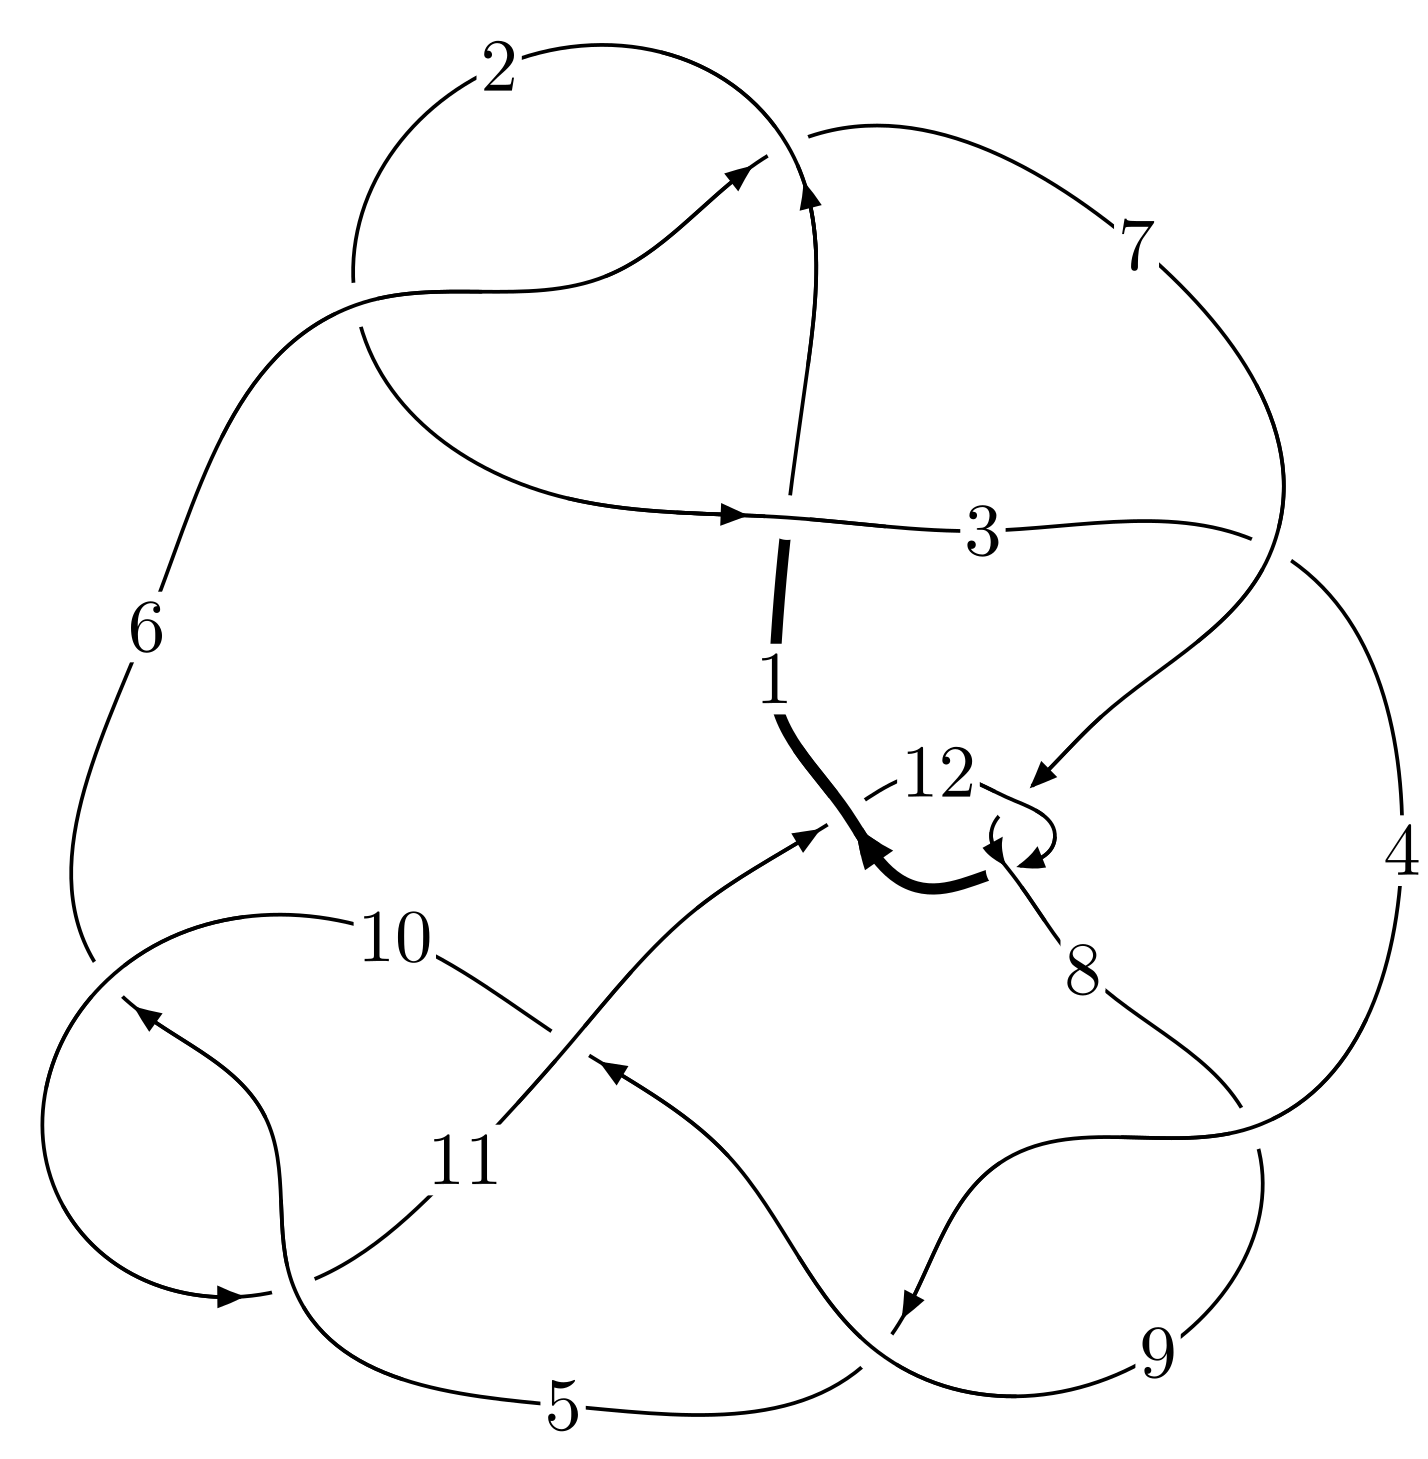
\includegraphics[width=112pt]{../../../GIT/diagram.site/Diagrams/png/1018_12a_0217.png}\\
\ \ \ A knot diagram\footnotemark}&
\allowdisplaybreaks
\textbf{Linearized knot diagam} \\
\cline{2-2}
 &
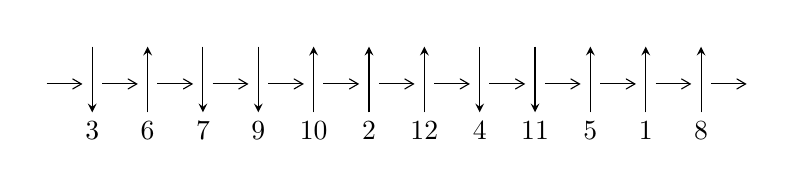
\begin{tikzpicture}[x=20pt, y=17pt]
	% nodes
	\node (C0) at (0, 0) {};
	\node (C1) at (1, 0) {};
	\node (C1U) at (1, +1) {};
	\node (C1D) at (1, -1) {3};

	\node (C2) at (2, 0) {};
	\node (C2U) at (2, +1) {};
	\node (C2D) at (2, -1) {6};

	\node (C3) at (3, 0) {};
	\node (C3U) at (3, +1) {};
	\node (C3D) at (3, -1) {7};

	\node (C4) at (4, 0) {};
	\node (C4U) at (4, +1) {};
	\node (C4D) at (4, -1) {9};

	\node (C5) at (5, 0) {};
	\node (C5U) at (5, +1) {};
	\node (C5D) at (5, -1) {10};

	\node (C6) at (6, 0) {};
	\node (C6U) at (6, +1) {};
	\node (C6D) at (6, -1) {2};

	\node (C7) at (7, 0) {};
	\node (C7U) at (7, +1) {};
	\node (C7D) at (7, -1) {12};

	\node (C8) at (8, 0) {};
	\node (C8U) at (8, +1) {};
	\node (C8D) at (8, -1) {4};

	\node (C9) at (9, 0) {};
	\node (C9U) at (9, +1) {};
	\node (C9D) at (9, -1) {11};

	\node (C10) at (10, 0) {};
	\node (C10U) at (10, +1) {};
	\node (C10D) at (10, -1) {5};

	\node (C11) at (11, 0) {};
	\node (C11U) at (11, +1) {};
	\node (C11D) at (11, -1) {1};

	\node (C12) at (12, 0) {};
	\node (C12U) at (12, +1) {};
	\node (C12D) at (12, -1) {8};
	\node (C13) at (13, 0) {};

	% arrows
	\draw[->,>={angle 60}]
	(C0) edge (C1) (C1) edge (C2) (C2) edge (C3) (C3) edge (C4) (C4) edge (C5) (C5) edge (C6) (C6) edge (C7) (C7) edge (C8) (C8) edge (C9) (C9) edge (C10) (C10) edge (C11) (C11) edge (C12) (C12) edge (C13) ;	\draw[->,>=stealth]
	(C1U) edge (C1D) (C2D) edge (C2U) (C3U) edge (C3D) (C4U) edge (C4D) (C5D) edge (C5U) (C6D) edge (C6U) (C7D) edge (C7U) (C8U) edge (C8D) (C9U) edge (C9D) (C10D) edge (C10U) (C11D) edge (C11U) (C12D) edge (C12U) ;
	\end{tikzpicture} \\
\hhline{~~} \\& 
\textbf{Solving Sequence} \\ \cline{2-2} 
 &
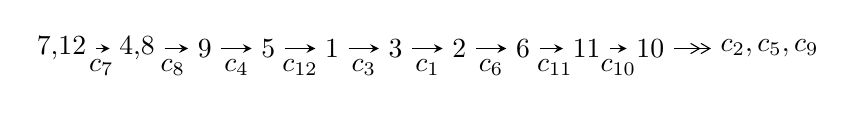
\begin{tikzpicture}[x=23pt, y=7pt]
	% node
	\node (A0) at (-1/8, 0) {7,12};
	\node (A1) at (17/16, 0) {4,8};
	\node (A2) at (17/8, 0) {9};
	\node (A3) at (25/8, 0) {5};
	\node (A4) at (33/8, 0) {1};
	\node (A5) at (41/8, 0) {3};
	\node (A6) at (49/8, 0) {2};
	\node (A7) at (57/8, 0) {6};
	\node (A8) at (65/8, 0) {11};
	\node (A9) at (73/8, 0) {10};
	\node (C1) at (1/2, -1) {$c_{7}$};
	\node (C2) at (13/8, -1) {$c_{8}$};
	\node (C3) at (21/8, -1) {$c_{4}$};
	\node (C4) at (29/8, -1) {$c_{12}$};
	\node (C5) at (37/8, -1) {$c_{3}$};
	\node (C6) at (45/8, -1) {$c_{1}$};
	\node (C7) at (53/8, -1) {$c_{6}$};
	\node (C8) at (61/8, -1) {$c_{11}$};
	\node (C9) at (69/8, -1) {$c_{10}$};
	\node (A10) at (11, 0) {$c_{2},c_{5},c_{9}$};

	% edge
	\draw[->,>=stealth]	
	(A0) edge (A1) (A1) edge (A2) (A2) edge (A3) (A3) edge (A4) (A4) edge (A5) (A5) edge (A6) (A6) edge (A7) (A7) edge (A8) (A8) edge (A9) ;
	\draw[->>,>={angle 60}]	
	(A9) edge (A10);
\end{tikzpicture} \\ 

\end{tabular} \\

\footnotetext{
The image of knot diagram is generated by the software ``\textbf{Draw programme}" developed by Andrew Bartholomew(\url{http://www.layer8.co.uk/maths/draw/index.htm\#Running-draw}), where we modified some parts for our purpose(\url{https://github.com/CATsTAILs/LinksPainter}).
}\phantom \\ \newline 
\centering \textbf{Ideals for irreducible components\footnotemark of $X_{\text{par}}$} 
 
\begin{align*}
I^u_{1}&=\langle 
3.70721\times10^{195} u^{111}+1.47324\times10^{196} u^{110}+\cdots+3.10521\times10^{195} b+1.11699\times10^{197},\\
\phantom{I^u_{1}}&\phantom{= \langle  }-2.13027\times10^{197} u^{111}-6.51014\times10^{197} u^{110}+\cdots+8.07355\times10^{196} a-3.95389\times10^{198},\\
\phantom{I^u_{1}}&\phantom{= \langle  }u^{112}+3 u^{111}+\cdots-15 u+13\rangle \\
I^u_{2}&=\langle 
76 a^7+266 a^6+388 a^5+305 a^4+824 a^3+1064 a^2+1105 b+204 a-624,\\
\phantom{I^u_{2}}&\phantom{= \langle  }a^8+4 a^7+6 a^6+4 a^5+9 a^4+16 a^3-4 a^2-12 a+13,\;u-1\rangle \\
I^u_{3}&=\langle 
2 a^5-5 a^4+10 a^3-10 a^2+3 b+10 a-2,\;a^6-3 a^5+6 a^4-7 a^3+6 a^2-3 a+1,\;u+1\rangle \\
\\
\end{align*}
\raggedright * 3 irreducible components of $\dim_{\mathbb{C}}=0$, with total 126 representations.\\
\footnotetext{All coefficients of polynomials are rational numbers. But the coefficients are sometimes approximated in decimal forms when there is not enough margin.}
\newpage
\renewcommand{\arraystretch}{1}
\centering \section*{I. $I^u_{1}= \langle 3.71\times10^{195} u^{111}+1.47\times10^{196} u^{110}+\cdots+3.11\times10^{195} b+1.12\times10^{197},\;-2.13\times10^{197} u^{111}-6.51\times10^{197} u^{110}+\cdots+8.07\times10^{196} a-3.95\times10^{198},\;u^{112}+3 u^{111}+\cdots-15 u+13 \rangle$}
\flushleft \textbf{(i) Arc colorings}\\
\begin{tabular}{m{7pt} m{180pt} m{7pt} m{180pt} }
\flushright $a_{7}=$&$\begin{pmatrix}1\\0\end{pmatrix}$ \\
\flushright $a_{12}=$&$\begin{pmatrix}0\\u\end{pmatrix}$ \\
\flushright $a_{4}=$&$\begin{pmatrix}2.63857 u^{111}+8.06354 u^{110}+\cdots-122.697 u+48.9733\\-1.19387 u^{111}-4.74441 u^{110}+\cdots+90.6056 u-35.9714\end{pmatrix}$ \\
\flushright $a_{8}=$&$\begin{pmatrix}1\\- u^2\end{pmatrix}$ \\
\flushright $a_{9}=$&$\begin{pmatrix}-2.99707 u^{111}-6.01775 u^{110}+\cdots+45.9311 u-22.1710\\2.77255 u^{111}+5.99213 u^{110}+\cdots-52.3866 u+32.6865\end{pmatrix}$ \\
\flushright $a_{5}=$&$\begin{pmatrix}0.435309 u^{111}+0.367120 u^{110}+\cdots+24.5090 u-6.98519\\-0.0312273 u^{111}-1.16652 u^{110}+\cdots+26.8632 u-5.19030\end{pmatrix}$ \\
\flushright $a_{1}=$&$\begin{pmatrix}u\\- u^3+u\end{pmatrix}$ \\
\flushright $a_{3}=$&$\begin{pmatrix}1.44470 u^{111}+3.31913 u^{110}+\cdots-32.0910 u+13.0019\\-1.19387 u^{111}-4.74441 u^{110}+\cdots+90.6056 u-35.9714\end{pmatrix}$ \\
\flushright $a_{2}=$&$\begin{pmatrix}1.04869 u^{111}+2.45896 u^{110}+\cdots-15.8751 u+5.26265\\0.166715 u^{111}-1.01686 u^{110}+\cdots+45.7581 u-16.0720\end{pmatrix}$ \\
\flushright $a_{6}=$&$\begin{pmatrix}1.75205 u^{111}+4.39266 u^{110}+\cdots-71.5032 u+30.3190\\-0.327588 u^{111}-2.29232 u^{110}+\cdots+70.4015 u-30.0065\end{pmatrix}$ \\
\flushright $a_{11}=$&$\begin{pmatrix}- u^3\\u^5- u^3+u\end{pmatrix}$ \\
\flushright $a_{10}=$&$\begin{pmatrix}0.172592 u^{111}+1.01161 u^{110}+\cdots-22.2733 u+16.4299\\3.14906 u^{111}+6.75817 u^{110}+\cdots-57.4630 u+36.9248\end{pmatrix}$\\&\end{tabular}
\flushleft \textbf{(ii) Obstruction class $= -1$}\\~\\
\flushleft \textbf{(iii) Cusp Shapes $= -0.990034 u^{111}-3.77498 u^{110}+\cdots+48.5280 u-1.50406$}\\~\\
\newpage\renewcommand{\arraystretch}{1}
\flushleft \textbf{(iv) u-Polynomials at the component}\newline \\
\begin{tabular}{m{50pt}|m{274pt}}
Crossings & \hspace{64pt}u-Polynomials at each crossing \\
\hline $$\begin{aligned}c_{1}\end{aligned}$$&$\begin{aligned}
&u^{112}+56 u^{111}+\cdots+8 u+1
\end{aligned}$\\
\hline $$\begin{aligned}c_{2},c_{6}\end{aligned}$$&$\begin{aligned}
&u^{112}-2 u^{111}+\cdots-2 u+1
\end{aligned}$\\
\hline $$\begin{aligned}c_{3}\end{aligned}$$&$\begin{aligned}
&u^{112}+2 u^{111}+\cdots-328230 u+69121
\end{aligned}$\\
\hline $$\begin{aligned}c_{4},c_{8}\end{aligned}$$&$\begin{aligned}
&u^{112}- u^{111}+\cdots+3468 u+548
\end{aligned}$\\
\hline $$\begin{aligned}c_{5},c_{10}\end{aligned}$$&$\begin{aligned}
&u^{112}+u^{111}+\cdots+4 u+4
\end{aligned}$\\
\hline $$\begin{aligned}c_{7},c_{12}\end{aligned}$$&$\begin{aligned}
&u^{112}-3 u^{111}+\cdots+15 u+13
\end{aligned}$\\
\hline $$\begin{aligned}c_{9}\end{aligned}$$&$\begin{aligned}
&u^{112}+61 u^{111}+\cdots+80 u+16
\end{aligned}$\\
\hline $$\begin{aligned}c_{11}\end{aligned}$$&$\begin{aligned}
&u^{112}-53 u^{111}+\cdots-1577 u+169
\end{aligned}$\\
\hline
\end{tabular}\\~\\
\newpage\renewcommand{\arraystretch}{1}
\flushleft \textbf{(v) Riley Polynomials at the component}\newline \\
\begin{tabular}{m{50pt}|m{274pt}}
Crossings & \hspace{64pt}Riley Polynomials at each crossing \\
\hline $$\begin{aligned}c_{1}\end{aligned}$$&$\begin{aligned}
&y^{112}+8 y^{111}+\cdots+56 y+1
\end{aligned}$\\
\hline $$\begin{aligned}c_{2},c_{6}\end{aligned}$$&$\begin{aligned}
&y^{112}+56 y^{111}+\cdots+8 y+1
\end{aligned}$\\
\hline $$\begin{aligned}c_{3}\end{aligned}$$&$\begin{aligned}
&y^{112}-40 y^{111}+\cdots-53022343592 y+4777712641
\end{aligned}$\\
\hline $$\begin{aligned}c_{4},c_{8}\end{aligned}$$&$\begin{aligned}
&y^{112}-91 y^{111}+\cdots+5715024 y+300304
\end{aligned}$\\
\hline $$\begin{aligned}c_{5},c_{10}\end{aligned}$$&$\begin{aligned}
&y^{112}+61 y^{111}+\cdots+80 y+16
\end{aligned}$\\
\hline $$\begin{aligned}c_{7},c_{12}\end{aligned}$$&$\begin{aligned}
&y^{112}-53 y^{111}+\cdots-1577 y+169
\end{aligned}$\\
\hline $$\begin{aligned}c_{9}\end{aligned}$$&$\begin{aligned}
&y^{112}-15 y^{111}+\cdots-5888 y+256
\end{aligned}$\\
\hline $$\begin{aligned}c_{11}\end{aligned}$$&$\begin{aligned}
&y^{112}+27 y^{111}+\cdots+1838795 y+28561
\end{aligned}$\\
\hline
\end{tabular}\\~\\
\newpage\flushleft \textbf{(vi) Complex Volumes and Cusp Shapes}
$$\begin{array}{c|c|c}  
\text{Solutions to }I^u_{1}& \I (\text{vol} + \sqrt{-1}CS) & \text{Cusp shape}\\
 \hline 
\begin{aligned}
u &= -0.450808 + 0.886061 I \\
a &= \phantom{-}0.385754 - 0.040786 I \\
b &= -1.27595 + 0.62290 I\end{aligned}
 & -6.67919 + 6.50991 I & \phantom{-0.000000 } 0 \\ \hline\begin{aligned}
u &= -0.450808 - 0.886061 I \\
a &= \phantom{-}0.385754 + 0.040786 I \\
b &= -1.27595 - 0.62290 I\end{aligned}
 & -6.67919 - 6.50991 I & \phantom{-0.000000 } 0 \\ \hline\begin{aligned}
u &= -0.857146 + 0.529607 I \\
a &= \phantom{-}1.30120 - 1.40188 I \\
b &= -0.70030 + 1.48450 I\end{aligned}
 & -2.77096 - 3.67618 I & \phantom{-0.000000 } 0 \\ \hline\begin{aligned}
u &= -0.857146 - 0.529607 I \\
a &= \phantom{-}1.30120 + 1.40188 I \\
b &= -0.70030 - 1.48450 I\end{aligned}
 & -2.77096 + 3.67618 I & \phantom{-0.000000 } 0 \\ \hline\begin{aligned}
u &= \phantom{-}0.982487 + 0.247895 I \\
a &= \phantom{-}1.327630 + 0.482226 I \\
b &= \phantom{-}0.239739 - 0.493297 I\end{aligned}
 & -0.50416 - 3.69973 I & \phantom{-0.000000 } 0 \\ \hline\begin{aligned}
u &= \phantom{-}0.982487 - 0.247895 I \\
a &= \phantom{-}1.327630 - 0.482226 I \\
b &= \phantom{-}0.239739 + 0.493297 I\end{aligned}
 & -0.50416 + 3.69973 I & \phantom{-0.000000 } 0 \\ \hline\begin{aligned}
u &= -0.542277 + 0.856250 I \\
a &= \phantom{-}0.410024 + 0.164661 I \\
b &= -1.317720 + 0.427134 I\end{aligned}
 & -7.27631 - 2.43835 I & \phantom{-0.000000 } 0 \\ \hline\begin{aligned}
u &= -0.542277 - 0.856250 I \\
a &= \phantom{-}0.410024 - 0.164661 I \\
b &= -1.317720 - 0.427134 I\end{aligned}
 & -7.27631 + 2.43835 I & \phantom{-0.000000 } 0 \\ \hline\begin{aligned}
u &= -0.859585 + 0.537868 I \\
a &= -0.62765 + 1.81967 I \\
b &= -0.16337 - 1.53346 I\end{aligned}
 & -2.75459 - 0.62134 I & \phantom{-0.000000 } 0 \\ \hline\begin{aligned}
u &= -0.859585 - 0.537868 I \\
a &= -0.62765 - 1.81967 I \\
b &= -0.16337 + 1.53346 I\end{aligned}
 & -2.75459 + 0.62134 I & \phantom{-0.000000 } 0\\
 \hline 
 \end{array}$$\newpage$$\begin{array}{c|c|c}  
\text{Solutions to }I^u_{1}& \I (\text{vol} + \sqrt{-1}CS) & \text{Cusp shape}\\
 \hline 
\begin{aligned}
u &= -0.924121 + 0.335108 I \\
a &= -0.886266 + 0.776763 I \\
b &= -0.493959 - 0.455629 I\end{aligned}
 & \phantom{-}1.76222 - 0.70527 I & \phantom{-0.000000 } 0 \\ \hline\begin{aligned}
u &= -0.924121 - 0.335108 I \\
a &= -0.886266 - 0.776763 I \\
b &= -0.493959 + 0.455629 I\end{aligned}
 & \phantom{-}1.76222 + 0.70527 I & \phantom{-0.000000 } 0 \\ \hline\begin{aligned}
u &= \phantom{-}0.827119 + 0.592053 I \\
a &= \phantom{-}0.084030 + 0.863952 I \\
b &= \phantom{-}1.010450 - 0.284902 I\end{aligned}
 & -2.31541 + 2.35649 I & \phantom{-0.000000 } 0 \\ \hline\begin{aligned}
u &= \phantom{-}0.827119 - 0.592053 I \\
a &= \phantom{-}0.084030 - 0.863952 I \\
b &= \phantom{-}1.010450 + 0.284902 I\end{aligned}
 & -2.31541 - 2.35649 I & \phantom{-0.000000 } 0 \\ \hline\begin{aligned}
u &= \phantom{-}0.716957 + 0.742374 I \\
a &= -0.111903 - 1.026480 I \\
b &= -1.094290 - 0.151911 I\end{aligned}
 & -5.89050 - 1.33250 I & \phantom{-0.000000 } 0 \\ \hline\begin{aligned}
u &= \phantom{-}0.716957 - 0.742374 I \\
a &= -0.111903 + 1.026480 I \\
b &= -1.094290 + 0.151911 I\end{aligned}
 & -5.89050 + 1.33250 I & \phantom{-0.000000 } 0 \\ \hline\begin{aligned}
u &= \phantom{-}0.432380 + 0.943489 I \\
a &= \phantom{-}0.070653 - 0.187610 I \\
b &= -1.49402 - 0.53409 I\end{aligned}
 & -6.28686 - 6.63610 I & \phantom{-0.000000 } 0 \\ \hline\begin{aligned}
u &= \phantom{-}0.432380 - 0.943489 I \\
a &= \phantom{-}0.070653 + 0.187610 I \\
b &= -1.49402 + 0.53409 I\end{aligned}
 & -6.28686 + 6.63610 I & \phantom{-0.000000 } 0 \\ \hline\begin{aligned}
u &= \phantom{-}0.825612 + 0.491984 I \\
a &= -1.32726 - 0.52908 I \\
b &= -0.998165 + 0.528922 I\end{aligned}
 & -2.45947 + 0.05845 I & \phantom{-0.000000 } 0 \\ \hline\begin{aligned}
u &= \phantom{-}0.825612 - 0.491984 I \\
a &= -1.32726 + 0.52908 I \\
b &= -0.998165 - 0.528922 I\end{aligned}
 & -2.45947 - 0.05845 I & \phantom{-0.000000 } 0\\
 \hline 
 \end{array}$$\newpage$$\begin{array}{c|c|c}  
\text{Solutions to }I^u_{1}& \I (\text{vol} + \sqrt{-1}CS) & \text{Cusp shape}\\
 \hline 
\begin{aligned}
u &= \phantom{-}0.473978 + 0.832935 I \\
a &= -0.307480 + 0.052481 I \\
b &= \phantom{-}1.207370 + 0.525705 I\end{aligned}
 & -3.39240 - 1.77371 I & \phantom{-0.000000 } 0 \\ \hline\begin{aligned}
u &= \phantom{-}0.473978 - 0.832935 I \\
a &= -0.307480 - 0.052481 I \\
b &= \phantom{-}1.207370 - 0.525705 I\end{aligned}
 & -3.39240 + 1.77371 I & \phantom{-0.000000 } 0 \\ \hline\begin{aligned}
u &= -0.902487 + 0.542851 I \\
a &= \phantom{-}0.983035 - 0.938609 I \\
b &= \phantom{-}1.122520 + 0.558603 I\end{aligned}
 & -0.48475 - 4.79014 I & \phantom{-0.000000 } 0 \\ \hline\begin{aligned}
u &= -0.902487 - 0.542851 I \\
a &= \phantom{-}0.983035 + 0.938609 I \\
b &= \phantom{-}1.122520 - 0.558603 I\end{aligned}
 & -0.48475 + 4.79014 I & \phantom{-0.000000 } 0 \\ \hline\begin{aligned}
u &= -0.787367 + 0.518126 I \\
a &= \phantom{-}0.28509 - 1.47521 I \\
b &= \phantom{-}0.749352 - 0.222493 I\end{aligned}
 & -0.866759 + 0.474494 I & \phantom{-0.000000 } 0 \\ \hline\begin{aligned}
u &= -0.787367 - 0.518126 I \\
a &= \phantom{-}0.28509 + 1.47521 I \\
b &= \phantom{-}0.749352 + 0.222493 I\end{aligned}
 & -0.866759 - 0.474494 I & \phantom{-0.000000 } 0 \\ \hline\begin{aligned}
u &= \phantom{-}0.916095 + 0.534423 I \\
a &= -0.05813 - 1.46802 I \\
b &= -0.638335 - 0.051172 I\end{aligned}
 & -2.10127 + 4.07115 I & \phantom{-0.000000 } 0 \\ \hline\begin{aligned}
u &= \phantom{-}0.916095 - 0.534423 I \\
a &= -0.05813 + 1.46802 I \\
b &= -0.638335 + 0.051172 I\end{aligned}
 & -2.10127 - 4.07115 I & \phantom{-0.000000 } 0 \\ \hline\begin{aligned}
u &= -0.408830 + 0.981568 I \\
a &= -0.152996 - 0.099204 I \\
b &= \phantom{-}1.55730 - 0.57237 I\end{aligned}
 & -9.5603 + 11.5301 I & \phantom{-0.000000 } 0 \\ \hline\begin{aligned}
u &= -0.408830 - 0.981568 I \\
a &= -0.152996 + 0.099204 I \\
b &= \phantom{-}1.55730 + 0.57237 I\end{aligned}
 & -9.5603 - 11.5301 I & \phantom{-0.000000 } 0\\
 \hline 
 \end{array}$$\newpage$$\begin{array}{c|c|c}  
\text{Solutions to }I^u_{1}& \I (\text{vol} + \sqrt{-1}CS) & \text{Cusp shape}\\
 \hline 
\begin{aligned}
u &= \phantom{-}0.940382 + 0.501312 I \\
a &= \phantom{-}0.71959 + 1.70667 I \\
b &= \phantom{-}0.02383 - 1.47836 I\end{aligned}
 & \phantom{-}0.90883 + 4.57646 I & \phantom{-0.000000 } 0 \\ \hline\begin{aligned}
u &= \phantom{-}0.940382 - 0.501312 I \\
a &= \phantom{-}0.71959 - 1.70667 I \\
b &= \phantom{-}0.02383 + 1.47836 I\end{aligned}
 & \phantom{-}0.90883 - 4.57646 I & \phantom{-0.000000 } 0 \\ \hline\begin{aligned}
u &= \phantom{-}0.817130 + 0.443293 I \\
a &= -1.22803 - 1.37489 I \\
b &= \phantom{-}0.63907 + 1.37754 I\end{aligned}
 & \phantom{-}0.390538 - 0.715302 I & \phantom{-0.000000 } 0 \\ \hline\begin{aligned}
u &= \phantom{-}0.817130 - 0.443293 I \\
a &= -1.22803 + 1.37489 I \\
b &= \phantom{-}0.63907 - 1.37754 I\end{aligned}
 & \phantom{-}0.390538 + 0.715302 I & \phantom{-0.000000 } 0 \\ \hline\begin{aligned}
u &= -0.486952 + 0.964165 I \\
a &= -0.163677 - 0.311624 I \\
b &= \phantom{-}1.52422 - 0.44200 I\end{aligned}
 & -10.37660 + 2.41346 I & \phantom{-0.000000 } 0 \\ \hline\begin{aligned}
u &= -0.486952 - 0.964165 I \\
a &= -0.163677 + 0.311624 I \\
b &= \phantom{-}1.52422 + 0.44200 I\end{aligned}
 & -10.37660 - 2.41346 I & \phantom{-0.000000 } 0 \\ \hline\begin{aligned}
u &= \phantom{-}0.628444 + 0.885268 I \\
a &= \phantom{-}0.095945 + 0.286157 I \\
b &= -1.066020 - 0.133992 I\end{aligned}
 & -7.62067 + 1.92280 I & \phantom{-0.000000 } 0 \\ \hline\begin{aligned}
u &= \phantom{-}0.628444 - 0.885268 I \\
a &= \phantom{-}0.095945 - 0.286157 I \\
b &= -1.066020 + 0.133992 I\end{aligned}
 & -7.62067 - 1.92280 I & \phantom{-0.000000 } 0 \\ \hline\begin{aligned}
u &= \phantom{-}1.068720 + 0.200240 I \\
a &= \phantom{-}0.771960 - 0.227365 I \\
b &= \phantom{-}0.007372 - 0.383032 I\end{aligned}
 & -1.16926 + 3.61056 I & \phantom{-0.000000 } 0 \\ \hline\begin{aligned}
u &= \phantom{-}1.068720 - 0.200240 I \\
a &= \phantom{-}0.771960 + 0.227365 I \\
b &= \phantom{-}0.007372 + 0.383032 I\end{aligned}
 & -1.16926 - 3.61056 I & \phantom{-0.000000 } 0\\
 \hline 
 \end{array}$$\newpage$$\begin{array}{c|c|c}  
\text{Solutions to }I^u_{1}& \I (\text{vol} + \sqrt{-1}CS) & \text{Cusp shape}\\
 \hline 
\begin{aligned}
u &= \phantom{-}1.058450 + 0.308302 I \\
a &= -1.24886 - 0.99979 I \\
b &= \phantom{-}0.880552 + 1.104800 I\end{aligned}
 & \phantom{-}2.38675 - 0.29739 I & \phantom{-0.000000 } 0 \\ \hline\begin{aligned}
u &= \phantom{-}1.058450 - 0.308302 I \\
a &= -1.24886 + 0.99979 I \\
b &= \phantom{-}0.880552 - 1.104800 I\end{aligned}
 & \phantom{-}2.38675 + 0.29739 I & \phantom{-0.000000 } 0 \\ \hline\begin{aligned}
u &= -0.595632 + 0.930937 I \\
a &= -0.176599 + 0.385479 I \\
b &= \phantom{-}1.043590 - 0.232052 I\end{aligned}
 & -11.13740 + 2.81193 I & \phantom{-0.000000 } 0 \\ \hline\begin{aligned}
u &= -0.595632 - 0.930937 I \\
a &= -0.176599 - 0.385479 I \\
b &= \phantom{-}1.043590 + 0.232052 I\end{aligned}
 & -11.13740 - 2.81193 I & \phantom{-0.000000 } 0 \\ \hline\begin{aligned}
u &= -0.964229 + 0.556788 I \\
a &= -0.79637 + 1.78638 I \\
b &= \phantom{-}0.01568 - 1.58229 I\end{aligned}
 & -2.19982 - 9.15039 I & \phantom{-0.000000 } 0 \\ \hline\begin{aligned}
u &= -0.964229 - 0.556788 I \\
a &= -0.79637 - 1.78638 I \\
b &= \phantom{-}0.01568 + 1.58229 I\end{aligned}
 & -2.19982 + 9.15039 I & \phantom{-0.000000 } 0 \\ \hline\begin{aligned}
u &= -0.710133 + 0.516149 I \\
a &= \phantom{-}1.22205 - 1.44142 I \\
b &= -0.51058 + 1.46382 I\end{aligned}
 & -3.04021 + 4.76122 I & \phantom{-0.000000 } 0 \\ \hline\begin{aligned}
u &= -0.710133 - 0.516149 I \\
a &= \phantom{-}1.22205 + 1.44142 I \\
b &= -0.51058 - 1.46382 I\end{aligned}
 & -3.04021 - 4.76122 I & \phantom{-0.000000 } 0 \\ \hline\begin{aligned}
u &= -1.026700 + 0.466594 I \\
a &= -0.61616 + 1.41099 I \\
b &= -0.760345 - 0.729067 I\end{aligned}
 & \phantom{-}2.85365 - 2.10734 I & \phantom{-0.000000 } 0 \\ \hline\begin{aligned}
u &= -1.026700 - 0.466594 I \\
a &= -0.61616 - 1.41099 I \\
b &= -0.760345 + 0.729067 I\end{aligned}
 & \phantom{-}2.85365 + 2.10734 I & \phantom{-0.000000 } 0\\
 \hline 
 \end{array}$$\newpage$$\begin{array}{c|c|c}  
\text{Solutions to }I^u_{1}& \I (\text{vol} + \sqrt{-1}CS) & \text{Cusp shape}\\
 \hline 
\begin{aligned}
u &= -0.683523 + 0.911532 I \\
a &= -0.196028 + 0.173729 I \\
b &= \phantom{-}1.175360 - 0.135200 I\end{aligned}
 & -11.47110 - 6.39364 I & \phantom{-0.000000 } 0 \\ \hline\begin{aligned}
u &= -0.683523 - 0.911532 I \\
a &= -0.196028 - 0.173729 I \\
b &= \phantom{-}1.175360 + 0.135200 I\end{aligned}
 & -11.47110 + 6.39364 I & \phantom{-0.000000 } 0 \\ \hline\begin{aligned}
u &= -1.128500 + 0.163734 I \\
a &= -0.975074 + 0.371373 I \\
b &= \phantom{-}0.244105 - 0.495902 I\end{aligned}
 & \phantom{-}2.03981 - 0.28607 I & \phantom{-0.000000 } 0 \\ \hline\begin{aligned}
u &= -1.128500 - 0.163734 I \\
a &= -0.975074 - 0.371373 I \\
b &= \phantom{-}0.244105 + 0.495902 I\end{aligned}
 & \phantom{-}2.03981 + 0.28607 I & \phantom{-0.000000 } 0 \\ \hline\begin{aligned}
u &= \phantom{-}1.077690 + 0.373170 I \\
a &= \phantom{-}0.89327 + 1.29029 I \\
b &= -0.224378 - 1.187290 I\end{aligned}
 & \phantom{-}3.45292 + 4.61019 I & \phantom{-0.000000 } 0 \\ \hline\begin{aligned}
u &= \phantom{-}1.077690 - 0.373170 I \\
a &= \phantom{-}0.89327 - 1.29029 I \\
b &= -0.224378 + 1.187290 I\end{aligned}
 & \phantom{-}3.45292 - 4.61019 I & \phantom{-0.000000 } 0 \\ \hline\begin{aligned}
u &= \phantom{-}0.935018 + 0.685604 I \\
a &= -0.261151 - 0.878476 I \\
b &= -1.319890 + 0.435228 I\end{aligned}
 & -5.24025 + 6.75819 I & \phantom{-0.000000 } 0 \\ \hline\begin{aligned}
u &= \phantom{-}0.935018 - 0.685604 I \\
a &= -0.261151 + 0.878476 I \\
b &= -1.319890 - 0.435228 I\end{aligned}
 & -5.24025 - 6.75819 I & \phantom{-0.000000 } 0 \\ \hline\begin{aligned}
u &= -1.124260 + 0.296257 I \\
a &= -0.957803 + 0.993983 I \\
b &= \phantom{-}0.299323 - 0.964655 I\end{aligned}
 & \phantom{-}3.69288 - 0.58388 I & \phantom{-0.000000 } 0 \\ \hline\begin{aligned}
u &= -1.124260 - 0.296257 I \\
a &= -0.957803 - 0.993983 I \\
b &= \phantom{-}0.299323 + 0.964655 I\end{aligned}
 & \phantom{-}3.69288 + 0.58388 I & \phantom{-0.000000 } 0\\
 \hline 
 \end{array}$$\newpage$$\begin{array}{c|c|c}  
\text{Solutions to }I^u_{1}& \I (\text{vol} + \sqrt{-1}CS) & \text{Cusp shape}\\
 \hline 
\begin{aligned}
u &= -1.159940 + 0.082093 I \\
a &= \phantom{-}0.428704 + 0.164622 I \\
b &= -0.485355 - 0.495379 I\end{aligned}
 & \phantom{-}0.70822 - 1.44061 I & \phantom{-0.000000 } 0 \\ \hline\begin{aligned}
u &= -1.159940 - 0.082093 I \\
a &= \phantom{-}0.428704 - 0.164622 I \\
b &= -0.485355 + 0.495379 I\end{aligned}
 & \phantom{-}0.70822 + 1.44061 I & \phantom{-0.000000 } 0 \\ \hline\begin{aligned}
u &= -1.034010 + 0.566715 I \\
a &= \phantom{-}0.57827 - 1.57727 I \\
b &= \phantom{-}1.28455 + 0.69444 I\end{aligned}
 & \phantom{-}0.58248 - 6.77944 I & \phantom{-0.000000 } 0 \\ \hline\begin{aligned}
u &= -1.034010 - 0.566715 I \\
a &= \phantom{-}0.57827 + 1.57727 I \\
b &= \phantom{-}1.28455 - 0.69444 I\end{aligned}
 & \phantom{-}0.58248 + 6.77944 I & \phantom{-0.000000 } 0 \\ \hline\begin{aligned}
u &= \phantom{-}1.070670 + 0.522453 I \\
a &= \phantom{-}0.41055 + 1.62106 I \\
b &= \phantom{-}0.896892 - 0.834838 I\end{aligned}
 & \phantom{-}2.17056 + 6.67494 I & \phantom{-0.000000 } 0 \\ \hline\begin{aligned}
u &= \phantom{-}1.070670 - 0.522453 I \\
a &= \phantom{-}0.41055 - 1.62106 I \\
b &= \phantom{-}0.896892 + 0.834838 I\end{aligned}
 & \phantom{-}2.17056 - 6.67494 I & \phantom{-0.000000 } 0 \\ \hline\begin{aligned}
u &= -1.172020 + 0.235636 I \\
a &= \phantom{-}1.27232 - 0.71187 I \\
b &= -0.972807 + 0.902220 I\end{aligned}
 & \phantom{-}2.30017 + 4.00091 I & \phantom{-0.000000 } 0 \\ \hline\begin{aligned}
u &= -1.172020 - 0.235636 I \\
a &= \phantom{-}1.27232 + 0.71187 I \\
b &= -0.972807 - 0.902220 I\end{aligned}
 & \phantom{-}2.30017 - 4.00091 I & \phantom{-0.000000 } 0 \\ \hline\begin{aligned}
u &= \phantom{-}1.201560 + 0.102438 I \\
a &= \phantom{-}1.293600 + 0.269876 I \\
b &= -0.508248 - 0.311304 I\end{aligned}
 & -0.78446 - 3.96097 I & \phantom{-0.000000 } 0 \\ \hline\begin{aligned}
u &= \phantom{-}1.201560 - 0.102438 I \\
a &= \phantom{-}1.293600 - 0.269876 I \\
b &= -0.508248 + 0.311304 I\end{aligned}
 & -0.78446 + 3.96097 I & \phantom{-0.000000 } 0\\
 \hline 
 \end{array}$$\newpage$$\begin{array}{c|c|c}  
\text{Solutions to }I^u_{1}& \I (\text{vol} + \sqrt{-1}CS) & \text{Cusp shape}\\
 \hline 
\begin{aligned}
u &= \phantom{-}0.381817 + 0.676898 I \\
a &= -0.724158 - 0.310670 I \\
b &= -1.116330 - 0.623866 I\end{aligned}
 & -2.13751 - 6.65846 I & -1.74684 + 7.19781 I \\ \hline\begin{aligned}
u &= \phantom{-}0.381817 - 0.676898 I \\
a &= -0.724158 + 0.310670 I \\
b &= -1.116330 + 0.623866 I\end{aligned}
 & -2.13751 + 6.65846 I & -1.74684 - 7.19781 I \\ \hline\begin{aligned}
u &= -0.530576 + 0.552072 I \\
a &= \phantom{-}0.821404 - 0.960181 I \\
b &= \phantom{-}0.941080 - 0.479178 I\end{aligned}
 & -0.90996 + 2.19304 I & \phantom{-0.000000 }      -6
0. 10   - 0.954685 I \\ \hline\begin{aligned}
u &= -0.530576 - 0.552072 I \\
a &= \phantom{-}0.821404 + 0.960181 I \\
b &= \phantom{-}0.941080 + 0.479178 I\end{aligned}
 & -0.90996 - 2.19304 I & \phantom{-0.000000 -}     -6
0. 10   + 0.954685 I \\ \hline\begin{aligned}
u &= \phantom{-}1.087630 + 0.588067 I \\
a &= -0.32008 - 1.75702 I \\
b &= -1.37091 + 0.74625 I\end{aligned}
 & -0.15222 + 11.58350 I & \phantom{-0.000000 } 0 \\ \hline\begin{aligned}
u &= \phantom{-}1.087630 - 0.588067 I \\
a &= -0.32008 + 1.75702 I \\
b &= -1.37091 - 0.74625 I\end{aligned}
 & -0.15222 - 11.58350 I & \phantom{-0.000000 } 0 \\ \hline\begin{aligned}
u &= \phantom{-}1.036770 + 0.726840 I \\
a &= \phantom{-}0.06854 - 1.43617 I \\
b &= -0.799763 + 0.348331 I\end{aligned}
 & -6.37547 + 4.01493 I & \phantom{-0.000000 } 0 \\ \hline\begin{aligned}
u &= \phantom{-}1.036770 - 0.726840 I \\
a &= \phantom{-}0.06854 + 1.43617 I \\
b &= -0.799763 - 0.348331 I\end{aligned}
 & -6.37547 - 4.01493 I & \phantom{-0.000000 } 0 \\ \hline\begin{aligned}
u &= -1.013590 + 0.772413 I \\
a &= -0.11678 - 1.41252 I \\
b &= \phantom{-}0.904586 + 0.355156 I\end{aligned}
 & -10.46070 + 0.23425 I & \phantom{-0.000000 } 0 \\ \hline\begin{aligned}
u &= -1.013590 - 0.772413 I \\
a &= -0.11678 + 1.41252 I \\
b &= \phantom{-}0.904586 - 0.355156 I\end{aligned}
 & -10.46070 - 0.23425 I & \phantom{-0.000000 } 0\\
 \hline 
 \end{array}$$\newpage$$\begin{array}{c|c|c}  
\text{Solutions to }I^u_{1}& \I (\text{vol} + \sqrt{-1}CS) & \text{Cusp shape}\\
 \hline 
\begin{aligned}
u &= -1.081080 + 0.678298 I \\
a &= \phantom{-}0.16557 + 1.64529 I \\
b &= -1.28240 - 0.82694 I\end{aligned}
 & -5.64478 - 3.26168 I & \phantom{-0.000000 } 0 \\ \hline\begin{aligned}
u &= -1.081080 - 0.678298 I \\
a &= \phantom{-}0.16557 - 1.64529 I \\
b &= -1.28240 + 0.82694 I\end{aligned}
 & -5.64478 + 3.26168 I & \phantom{-0.000000 } 0 \\ \hline\begin{aligned}
u &= \phantom{-}1.106860 + 0.643894 I \\
a &= -0.05335 + 1.74699 I \\
b &= \phantom{-}1.20472 - 0.90179 I\end{aligned}
 & -1.48775 + 7.29013 I & \phantom{-0.000000 } 0 \\ \hline\begin{aligned}
u &= \phantom{-}1.106860 - 0.643894 I \\
a &= -0.05335 - 1.74699 I \\
b &= \phantom{-}1.20472 + 0.90179 I\end{aligned}
 & -1.48775 - 7.29013 I & \phantom{-0.000000 } 0 \\ \hline\begin{aligned}
u &= \phantom{-}0.703712 + 0.100809 I \\
a &= -0.29810 + 1.73880 I \\
b &= \phantom{-}0.412036 - 1.130510 I\end{aligned}
 & \phantom{-}0.64540 + 2.34760 I & -3.30070 - 5.06400 I \\ \hline\begin{aligned}
u &= \phantom{-}0.703712 - 0.100809 I \\
a &= -0.29810 - 1.73880 I \\
b &= \phantom{-}0.412036 + 1.130510 I\end{aligned}
 & \phantom{-}0.64540 - 2.34760 I & -3.30070 + 5.06400 I \\ \hline\begin{aligned}
u &= -1.074640 + 0.737016 I \\
a &= -0.07256 - 1.47431 I \\
b &= \phantom{-}0.775909 + 0.426799 I\end{aligned}
 & -9.67145 - 8.90991 I & \phantom{-0.000000 } 0 \\ \hline\begin{aligned}
u &= -1.074640 - 0.737016 I \\
a &= -0.07256 + 1.47431 I \\
b &= \phantom{-}0.775909 - 0.426799 I\end{aligned}
 & -9.67145 + 8.90991 I & \phantom{-0.000000 } 0 \\ \hline\begin{aligned}
u &= -1.133230 + 0.656462 I \\
a &= \phantom{-}0.10862 + 1.83683 I \\
b &= -1.24411 - 0.96475 I\end{aligned}
 & -4.61274 - 12.20790 I & \phantom{-0.000000 } 0 \\ \hline\begin{aligned}
u &= -1.133230 - 0.656462 I \\
a &= \phantom{-}0.10862 - 1.83683 I \\
b &= -1.24411 + 0.96475 I\end{aligned}
 & -4.61274 + 12.20790 I & \phantom{-0.000000 } 0\\
 \hline 
 \end{array}$$\newpage$$\begin{array}{c|c|c}  
\text{Solutions to }I^u_{1}& \I (\text{vol} + \sqrt{-1}CS) & \text{Cusp shape}\\
 \hline 
\begin{aligned}
u &= -1.320560 + 0.108558 I \\
a &= \phantom{-}1.293560 - 0.189033 I \\
b &= -1.047620 + 0.519491 I\end{aligned}
 & -0.01600 + 3.48973 I & \phantom{-0.000000 } 0 \\ \hline\begin{aligned}
u &= -1.320560 - 0.108558 I \\
a &= \phantom{-}1.293560 + 0.189033 I \\
b &= -1.047620 - 0.519491 I\end{aligned}
 & -0.01600 - 3.48973 I & \phantom{-0.000000 } 0 \\ \hline\begin{aligned}
u &= \phantom{-}1.158700 + 0.671263 I \\
a &= \phantom{-}0.21640 - 1.77484 I \\
b &= -1.57741 + 0.75572 I\end{aligned}
 & -4.07231 + 12.53520 I & \phantom{-0.000000 } 0 \\ \hline\begin{aligned}
u &= \phantom{-}1.158700 - 0.671263 I \\
a &= \phantom{-}0.21640 + 1.77484 I \\
b &= -1.57741 - 0.75572 I\end{aligned}
 & -4.07231 - 12.53520 I & \phantom{-0.000000 } 0 \\ \hline\begin{aligned}
u &= -1.143650 + 0.704530 I \\
a &= -0.28766 - 1.62742 I \\
b &= \phantom{-}1.60927 + 0.69063 I\end{aligned}
 & -8.36778 - 8.49053 I & \phantom{-0.000000 } 0 \\ \hline\begin{aligned}
u &= -1.143650 - 0.704530 I \\
a &= -0.28766 + 1.62742 I \\
b &= \phantom{-}1.60927 - 0.69063 I\end{aligned}
 & -8.36778 + 8.49053 I & \phantom{-0.000000 } 0 \\ \hline\begin{aligned}
u &= \phantom{-}1.356570 + 0.058794 I \\
a &= -1.273020 - 0.006187 I \\
b &= \phantom{-}1.036810 + 0.381627 I\end{aligned}
 & -3.58530 + 0.61655 I & \phantom{-0.000000 } 0 \\ \hline\begin{aligned}
u &= \phantom{-}1.356570 - 0.058794 I \\
a &= -1.273020 + 0.006187 I \\
b &= \phantom{-}1.036810 - 0.381627 I\end{aligned}
 & -3.58530 - 0.61655 I & \phantom{-0.000000 } 0 \\ \hline\begin{aligned}
u &= -1.182990 + 0.675532 I \\
a &= -0.30380 - 1.84456 I \\
b &= \phantom{-}1.61431 + 0.78845 I\end{aligned}
 & -7.1880 - 17.5468 I & \phantom{-0.000000 } 0 \\ \hline\begin{aligned}
u &= -1.182990 - 0.675532 I \\
a &= -0.30380 + 1.84456 I \\
b &= \phantom{-}1.61431 - 0.78845 I\end{aligned}
 & -7.1880 + 17.5468 I & \phantom{-0.000000 } 0\\
 \hline 
 \end{array}$$\newpage$$\begin{array}{c|c|c}  
\text{Solutions to }I^u_{1}& \I (\text{vol} + \sqrt{-1}CS) & \text{Cusp shape}\\
 \hline 
\begin{aligned}
u &= \phantom{-}0.225025 + 0.596399 I \\
a &= \phantom{-}0.286234 - 0.057094 I \\
b &= \phantom{-}0.578271 + 0.650812 I\end{aligned}
 & -0.04328 - 2.34631 I & \phantom{-}1.81701 + 3.47116 I \\ \hline\begin{aligned}
u &= \phantom{-}0.225025 - 0.596399 I \\
a &= \phantom{-}0.286234 + 0.057094 I \\
b &= \phantom{-}0.578271 - 0.650812 I\end{aligned}
 & -0.04328 + 2.34631 I & \phantom{-}1.81701 - 3.47116 I \\ \hline\begin{aligned}
u &= \phantom{-}0.221549 + 0.591679 I \\
a &= -0.140575 + 1.066260 I \\
b &= -0.340236 + 0.151538 I\end{aligned}
 & -3.63686 - 0.52707 I & -7.64565 + 0.08563 I \\ \hline\begin{aligned}
u &= \phantom{-}0.221549 - 0.591679 I \\
a &= -0.140575 - 1.066260 I \\
b &= -0.340236 - 0.151538 I\end{aligned}
 & -3.63686 + 0.52707 I & -7.64565 - 0.08563 I \\ \hline\begin{aligned}
u &= \phantom{-}1.363180 + 0.136144 I \\
a &= -1.43861 - 0.16525 I \\
b &= \phantom{-}1.159640 + 0.507977 I\end{aligned}
 & -3.22973 - 7.98182 I & \phantom{-0.000000 } 0 \\ \hline\begin{aligned}
u &= \phantom{-}1.363180 - 0.136144 I \\
a &= -1.43861 + 0.16525 I \\
b &= \phantom{-}1.159640 - 0.507977 I\end{aligned}
 & -3.22973 + 7.98182 I & \phantom{-0.000000 } 0 \\ \hline\begin{aligned}
u &= -0.048150 + 0.456195 I \\
a &= -0.826428 + 0.180873 I \\
b &= -0.134291 + 0.725341 I\end{aligned}
 & \phantom{-}0.61726 - 1.41846 I & \phantom{-}3.09666 + 4.67925 I \\ \hline\begin{aligned}
u &= -0.048150 - 0.456195 I \\
a &= -0.826428 - 0.180873 I \\
b &= -0.134291 - 0.725341 I\end{aligned}
 & \phantom{-}0.61726 + 1.41846 I & \phantom{-}3.09666 - 4.67925 I \\ \hline\begin{aligned}
u &= \phantom{-}0.396967 + 0.201628 I \\
a &= -1.33484 + 2.21073 I \\
b &= -0.567097 + 0.562797 I\end{aligned}
 & -2.48400 + 6.00879 I & -4.68112 - 8.65446 I \\ \hline\begin{aligned}
u &= \phantom{-}0.396967 - 0.201628 I \\
a &= -1.33484 - 2.21073 I \\
b &= -0.567097 - 0.562797 I\end{aligned}
 & -2.48400 - 6.00879 I & -4.68112 + 8.65446 I\\
 \hline 
 \end{array}$$\newpage$$\begin{array}{c|c|c}  
\text{Solutions to }I^u_{1}& \I (\text{vol} + \sqrt{-1}CS) & \text{Cusp shape}\\
 \hline 
\begin{aligned}
u &= -0.164490 + 0.292346 I \\
a &= -0.48184 + 2.19627 I \\
b &= \phantom{-}0.345986 + 0.586919 I\end{aligned}
 & -0.32189 - 1.84668 I & -0.17990 + 4.47002 I \\ \hline\begin{aligned}
u &= -0.164490 - 0.292346 I \\
a &= -0.48184 - 2.19627 I \\
b &= \phantom{-}0.345986 - 0.586919 I\end{aligned}
 & -0.32189 + 1.84668 I & -0.17990 - 4.47002 I\\
 \hline 
 \end{array}$$\newpage\newpage\renewcommand{\arraystretch}{1}
\centering \section*{II. $I^u_{2}= \langle 76 a^7+1105 b+\cdots+204 a-624,\;a^8+4 a^7+\cdots-12 a+13,\;u-1 \rangle$}
\flushleft \textbf{(i) Arc colorings}\\
\begin{tabular}{m{7pt} m{180pt} m{7pt} m{180pt} }
\flushright $a_{7}=$&$\begin{pmatrix}1\\0\end{pmatrix}$ \\
\flushright $a_{12}=$&$\begin{pmatrix}0\\1\end{pmatrix}$ \\
\flushright $a_{4}=$&$\begin{pmatrix}a\\-0.0687783 a^{7}-0.240724 a^{6}+\cdots-0.184615 a+0.564706\end{pmatrix}$ \\
\flushright $a_{8}=$&$\begin{pmatrix}1\\-1\end{pmatrix}$ \\
\flushright $a_{9}=$&$\begin{pmatrix}0.0343891 a^{7}+0.0615385 a^{6}+\cdots-0.260633 a+1.89412\\-0.0343891 a^{7}-0.179186 a^{6}+\cdots-0.445249 a-0.541176\end{pmatrix}$ \\
\flushright $a_{5}=$&$\begin{pmatrix}0.186425 a^{7}+0.593665 a^{6}+\cdots-1.16833 a-0.564706\\-0.130317 a^{7}-0.397285 a^{6}+\cdots+1.84525 a+0.788235\end{pmatrix}$ \\
\flushright $a_{1}=$&$\begin{pmatrix}1\\0\end{pmatrix}$ \\
\flushright $a_{3}=$&$\begin{pmatrix}-0.0687783 a^{7}-0.240724 a^{6}+\cdots+0.815385 a+0.564706\\-0.0687783 a^{7}-0.240724 a^{6}+\cdots-0.184615 a+0.564706\end{pmatrix}$ \\
\flushright $a_{2}=$&$\begin{pmatrix}-0.0343891 a^{7}-0.179186 a^{6}+\cdots-0.445249 a+1.45882\\-0.0687783 a^{7}-0.240724 a^{6}+\cdots-0.184615 a-0.435294\end{pmatrix}$ \\
\flushright $a_{6}=$&$\begin{pmatrix}- a\\0.0687783 a^{7}+0.240724 a^{6}+\cdots+0.184615 a-0.564706\end{pmatrix}$ \\
\flushright $a_{11}=$&$\begin{pmatrix}-1\\1\end{pmatrix}$ \\
\flushright $a_{10}=$&$\begin{pmatrix}0.0343891 a^{7}+0.179186 a^{6}+\cdots+0.445249 a+0.541176\\-0.0343891 a^{7}-0.296833 a^{6}+\cdots-1.15113 a+0.811765\end{pmatrix}$\\&\end{tabular}
\flushleft \textbf{(ii) Obstruction class $= 1$}\\~\\
\flushleft \textbf{(iii) Cusp Shapes $= -\frac{304}{1105} a^7-\frac{1584}{1105} a^6-\frac{3112}{1105} a^5-\frac{712}{221} a^4-\frac{5376}{1105} a^3-\frac{8156}{1105} a^2-\frac{3936}{1105} a+\frac{312}{85}$}\\~\\
\newpage\renewcommand{\arraystretch}{1}
\flushleft \textbf{(iv) u-Polynomials at the component}\newline \\
\begin{tabular}{m{50pt}|m{274pt}}
Crossings & \hspace{64pt}u-Polynomials at each crossing \\
\hline $$\begin{aligned}c_{1},c_{2}\end{aligned}$$&$\begin{aligned}
&(u^2- u+1)^4
\end{aligned}$\\
\hline $$\begin{aligned}c_{3},c_{6}\end{aligned}$$&$\begin{aligned}
&(u^2+u+1)^4
\end{aligned}$\\
\hline $$\begin{aligned}c_{4},c_{8}\end{aligned}$$&$\begin{aligned}
&(u^4-2 u^2+2)^2
\end{aligned}$\\
\hline $$\begin{aligned}c_{5},c_{10}\end{aligned}$$&$\begin{aligned}
&(u^4+2 u^2+2)^2
\end{aligned}$\\
\hline $$\begin{aligned}c_{7}\end{aligned}$$&$\begin{aligned}
&(u-1)^8
\end{aligned}$\\
\hline $$\begin{aligned}c_{9}\end{aligned}$$&$\begin{aligned}
&(u^2-2 u+2)^4
\end{aligned}$\\
\hline $$\begin{aligned}c_{11},c_{12}\end{aligned}$$&$\begin{aligned}
&(u+1)^8
\end{aligned}$\\
\hline
\end{tabular}\\~\\
\newpage\renewcommand{\arraystretch}{1}
\flushleft \textbf{(v) Riley Polynomials at the component}\newline \\
\begin{tabular}{m{50pt}|m{274pt}}
Crossings & \hspace{64pt}Riley Polynomials at each crossing \\
\hline $$\begin{aligned}c_{1},c_{2},c_{3}\\c_{6}\end{aligned}$$&$\begin{aligned}
&(y^2+y+1)^4
\end{aligned}$\\
\hline $$\begin{aligned}c_{4},c_{8}\end{aligned}$$&$\begin{aligned}
&(y^2-2 y+2)^4
\end{aligned}$\\
\hline $$\begin{aligned}c_{5},c_{10}\end{aligned}$$&$\begin{aligned}
&(y^2+2 y+2)^4
\end{aligned}$\\
\hline $$\begin{aligned}c_{7},c_{11},c_{12}\end{aligned}$$&$\begin{aligned}
&(y-1)^8
\end{aligned}$\\
\hline $$\begin{aligned}c_{9}\end{aligned}$$&$\begin{aligned}
&(y^2+4)^4
\end{aligned}$\\
\hline
\end{tabular}\\~\\
\newpage\flushleft \textbf{(vi) Complex Volumes and Cusp Shapes}
$$\begin{array}{c|c|c}  
\text{Solutions to }I^u_{2}& \I (\text{vol} + \sqrt{-1}CS) & \text{Cusp shape}\\
 \hline 
\begin{aligned}
u &= \phantom{-}1.00000\phantom{ +0.000000I} \\
a &= \phantom{-}0.598684 + 0.410936 I \\
b &= \phantom{-}0.500000 - 0.866025 I\end{aligned}
 & -0.82247 + 5.69375 I & \phantom{-}2.00000 - 7.46410 I \\ \hline\begin{aligned}
u &= \phantom{-}1.00000\phantom{ +0.000000I} \\
a &= \phantom{-}0.598684 - 0.410936 I \\
b &= \phantom{-}0.500000 + 0.866025 I\end{aligned}
 & -0.82247 - 5.69375 I & \phantom{-}2.00000 + 7.46410 I \\ \hline\begin{aligned}
u &= \phantom{-}1.00000\phantom{ +0.000000I} \\
a &= \phantom{-}0.59868 + 1.32112 I \\
b &= \phantom{-}0.500000 - 0.866025 I\end{aligned}
 & -0.82247 - 1.63398 I & \phantom{-}2.00000 + 0.53590 I \\ \hline\begin{aligned}
u &= \phantom{-}1.00000\phantom{ +0.000000I} \\
a &= \phantom{-}0.59868 - 1.32112 I \\
b &= \phantom{-}0.500000 + 0.866025 I\end{aligned}
 & -0.82247 + 1.63398 I & \phantom{-}2.00000 - 0.53590 I \\ \hline\begin{aligned}
u &= \phantom{-}1.00000\phantom{ +0.000000I} \\
a &= -1.59868 + 0.41094 I \\
b &= \phantom{-}0.500000 - 0.866025 I\end{aligned}
 & -0.82247 - 1.63398 I & \phantom{-}2.00000 + 0.53590 I \\ \hline\begin{aligned}
u &= \phantom{-}1.00000\phantom{ +0.000000I} \\
a &= -1.59868 - 0.41094 I \\
b &= \phantom{-}0.500000 + 0.866025 I\end{aligned}
 & -0.82247 + 1.63398 I & \phantom{-}2.00000 - 0.53590 I \\ \hline\begin{aligned}
u &= \phantom{-}1.00000\phantom{ +0.000000I} \\
a &= -1.59868 + 1.32112 I \\
b &= \phantom{-}0.500000 - 0.866025 I\end{aligned}
 & -0.82247 + 5.69375 I & \phantom{-}2.00000 - 7.46410 I \\ \hline\begin{aligned}
u &= \phantom{-}1.00000\phantom{ +0.000000I} \\
a &= -1.59868 - 1.32112 I \\
b &= \phantom{-}0.500000 + 0.866025 I\end{aligned}
 & -0.82247 - 5.69375 I & \phantom{-}2.00000 + 7.46410 I\\
 \hline 
 \end{array}$$\newpage\newpage\renewcommand{\arraystretch}{1}
\centering \section*{III. $I^u_{3}= \langle 2 a^5-5 a^4+10 a^3-10 a^2+3 b+10 a-2,\;a^6-3 a^5+6 a^4-7 a^3+6 a^2-3 a+1,\;u+1 \rangle$}
\flushleft \textbf{(i) Arc colorings}\\
\begin{tabular}{m{7pt} m{180pt} m{7pt} m{180pt} }
\flushright $a_{7}=$&$\begin{pmatrix}1\\0\end{pmatrix}$ \\
\flushright $a_{12}=$&$\begin{pmatrix}0\\-1\end{pmatrix}$ \\
\flushright $a_{4}=$&$\begin{pmatrix}a\\-\frac{2}{3} a^5+\frac{5}{3} a^4+\cdots-\frac{10}{3} a+\frac{2}{3}\end{pmatrix}$ \\
\flushright $a_{8}=$&$\begin{pmatrix}1\\-1\end{pmatrix}$ \\
\flushright $a_{9}=$&$\begin{pmatrix}-\frac{1}{3} a^5+\frac{2}{3} a^4+\cdots-\frac{4}{3} a+\frac{5}{3}\\\frac{1}{3} a^5- a^4+2 a^3-\frac{8}{3} a^2+2 a-2\end{pmatrix}$ \\
\flushright $a_{5}=$&$\begin{pmatrix}a^5-\frac{7}{3} a^4+\cdots+\frac{11}{3} a-\frac{2}{3}\\-\frac{5}{3} a^5+4 a^4+\cdots-6 a+\frac{4}{3}\end{pmatrix}$ \\
\flushright $a_{1}=$&$\begin{pmatrix}-1\\0\end{pmatrix}$ \\
\flushright $a_{3}=$&$\begin{pmatrix}-\frac{2}{3} a^5+\frac{5}{3} a^4+\cdots-\frac{7}{3} a+\frac{2}{3}\\-\frac{2}{3} a^5+\frac{5}{3} a^4+\cdots-\frac{10}{3} a+\frac{2}{3}\end{pmatrix}$ \\
\flushright $a_{2}=$&$\begin{pmatrix}-\frac{1}{3} a^5+a^4-2 a^3+\frac{8}{3} a^2-2 a\\-\frac{2}{3} a^5+\frac{5}{3} a^4+\cdots-\frac{10}{3} a+\frac{5}{3}\end{pmatrix}$ \\
\flushright $a_{6}=$&$\begin{pmatrix}a\\-\frac{2}{3} a^5+\frac{5}{3} a^4+\cdots-\frac{10}{3} a+\frac{2}{3}\end{pmatrix}$ \\
\flushright $a_{11}=$&$\begin{pmatrix}1\\-1\end{pmatrix}$ \\
\flushright $a_{10}=$&$\begin{pmatrix}-\frac{1}{3} a^5+a^4-2 a^3+\frac{8}{3} a^2-2 a+2\\\frac{1}{3} a^5-\frac{4}{3} a^4+\cdots+\frac{8}{3} a-\frac{7}{3}\end{pmatrix}$\\&\end{tabular}
\flushleft \textbf{(ii) Obstruction class $= 1$}\\~\\
\flushleft \textbf{(iii) Cusp Shapes $= \frac{8}{3} a^5-6 a^4+12 a^3-\frac{34}{3} a^2+12 a+2$}\\~\\
\newpage\renewcommand{\arraystretch}{1}
\flushleft \textbf{(iv) u-Polynomials at the component}\newline \\
\begin{tabular}{m{50pt}|m{274pt}}
Crossings & \hspace{64pt}u-Polynomials at each crossing \\
\hline $$\begin{aligned}c_{1},c_{3},c_{6}\end{aligned}$$&$\begin{aligned}
&(u^2- u+1)^3
\end{aligned}$\\
\hline $$\begin{aligned}c_{2}\end{aligned}$$&$\begin{aligned}
&(u^2+u+1)^3
\end{aligned}$\\
\hline $$\begin{aligned}c_{4},c_{5},c_{8}\\c_{9},c_{10}\end{aligned}$$&$\begin{aligned}
&u^6
\end{aligned}$\\
\hline $$\begin{aligned}c_{7},c_{11}\end{aligned}$$&$\begin{aligned}
&(u+1)^6
\end{aligned}$\\
\hline $$\begin{aligned}c_{12}\end{aligned}$$&$\begin{aligned}
&(u-1)^6
\end{aligned}$\\
\hline
\end{tabular}\\~\\
\newpage\renewcommand{\arraystretch}{1}
\flushleft \textbf{(v) Riley Polynomials at the component}\newline \\
\begin{tabular}{m{50pt}|m{274pt}}
Crossings & \hspace{64pt}Riley Polynomials at each crossing \\
\hline $$\begin{aligned}c_{1},c_{2},c_{3}\\c_{6}\end{aligned}$$&$\begin{aligned}
&(y^2+y+1)^3
\end{aligned}$\\
\hline $$\begin{aligned}c_{4},c_{5},c_{8}\\c_{9},c_{10}\end{aligned}$$&$\begin{aligned}
&y^6
\end{aligned}$\\
\hline $$\begin{aligned}c_{7},c_{11},c_{12}\end{aligned}$$&$\begin{aligned}
&(y-1)^6
\end{aligned}$\\
\hline
\end{tabular}\\~\\
\newpage\flushleft \textbf{(vi) Complex Volumes and Cusp Shapes}
$$\begin{array}{c|c|c}  
\text{Solutions to }I^u_{3}& \I (\text{vol} + \sqrt{-1}CS) & \text{Cusp shape}\\
 \hline 
\begin{aligned}
u &= -1.00000\phantom{ +0.000000I} \\
a &= \phantom{-}0.500000 + 0.866025 I \\
b &= -0.500000 - 0.866025 I\end{aligned}
 & \phantom{-}1.64493 - 2.02988 I & \phantom{-}6.00000 + 3.46410 I \\ \hline\begin{aligned}
u &= -1.00000\phantom{ +0.000000I} \\
a &= \phantom{-}0.500000 + 0.866025 I \\
b &= -0.500000 - 0.866025 I\end{aligned}
 & \phantom{-}1.64493 - 2.02988 I & \phantom{-}6.00000 + 3.46410 I \\ \hline\begin{aligned}
u &= -1.00000\phantom{ +0.000000I} \\
a &= \phantom{-}0.500000 + 0.866025 I \\
b &= -0.500000 - 0.866025 I\end{aligned}
 & \phantom{-}1.64493 - 2.02988 I & \phantom{-}6.00000 + 3.46410 I \\ \hline\begin{aligned}
u &= -1.00000\phantom{ +0.000000I} \\
a &= \phantom{-}0.500000 - 0.866025 I \\
b &= -0.500000 + 0.866025 I\end{aligned}
 & \phantom{-}1.64493 + 2.02988 I & \phantom{-}6.00000 - 3.46410 I \\ \hline\begin{aligned}
u &= -1.00000\phantom{ +0.000000I} \\
a &= \phantom{-}0.500000 - 0.866025 I \\
b &= -0.500000 + 0.866025 I\end{aligned}
 & \phantom{-}1.64493 + 2.02988 I & \phantom{-}6.00000 - 3.46410 I \\ \hline\begin{aligned}
u &= -1.00000\phantom{ +0.000000I} \\
a &= \phantom{-}0.500000 - 0.866025 I \\
b &= -0.500000 + 0.866025 I\end{aligned}
 & \phantom{-}1.64493 + 2.02988 I & \phantom{-}6.00000 - 3.46410 I\\
 \hline 
 \end{array}$$\newpage
\newpage\renewcommand{\arraystretch}{1}
\centering \section*{ IV. u-Polynomials}
\begin{tabular}{m{50pt}|m{274pt}}
Crossings & \hspace{64pt}u-Polynomials at each crossing \\
\hline $$\begin{aligned}c_{1}\end{aligned}$$&$\begin{aligned}
&((u^2- u+1)^7)(u^{112}+56 u^{111}+\cdots+8 u+1)
\end{aligned}$\\
\hline $$\begin{aligned}c_{2}\end{aligned}$$&$\begin{aligned}
&((u^2- u+1)^4)(u^2+u+1)^3(u^{112}-2 u^{111}+\cdots-2 u+1)
\end{aligned}$\\
\hline $$\begin{aligned}c_{3}\end{aligned}$$&$\begin{aligned}
&((u^2- u+1)^3)(u^2+u+1)^4(u^{112}+2 u^{111}+\cdots-328230 u+69121)
\end{aligned}$\\
\hline $$\begin{aligned}c_{4},c_{8}\end{aligned}$$&$\begin{aligned}
&u^6(u^4-2 u^2+2)^2(u^{112}-u^{111}+\cdots+3468 u+548)
\end{aligned}$\\
\hline $$\begin{aligned}c_{5},c_{10}\end{aligned}$$&$\begin{aligned}
&u^6(u^4+2 u^2+2)^2(u^{112}+u^{111}+\cdots+4 u+4)
\end{aligned}$\\
\hline $$\begin{aligned}c_{6}\end{aligned}$$&$\begin{aligned}
&((u^2- u+1)^3)(u^2+u+1)^4(u^{112}-2 u^{111}+\cdots-2 u+1)
\end{aligned}$\\
\hline $$\begin{aligned}c_{7}\end{aligned}$$&$\begin{aligned}
&((u-1)^8)(u+1)^6(u^{112}-3 u^{111}+\cdots+15 u+13)
\end{aligned}$\\
\hline $$\begin{aligned}c_{9}\end{aligned}$$&$\begin{aligned}
&u^6(u^2-2 u+2)^4(u^{112}+61 u^{111}+\cdots+80 u+16)
\end{aligned}$\\
\hline $$\begin{aligned}c_{11}\end{aligned}$$&$\begin{aligned}
&((u+1)^{14})(u^{112}-53 u^{111}+\cdots-1577 u+169)
\end{aligned}$\\
\hline $$\begin{aligned}c_{12}\end{aligned}$$&$\begin{aligned}
&((u-1)^6)(u+1)^8(u^{112}-3 u^{111}+\cdots+15 u+13)
\end{aligned}$\\
\hline
\end{tabular}\newpage\renewcommand{\arraystretch}{1}
\centering \section*{ V. Riley Polynomials}
\begin{tabular}{m{50pt}|m{274pt}}
Crossings & \hspace{64pt}Riley Polynomials at each crossing \\
\hline $$\begin{aligned}c_{1}\end{aligned}$$&$\begin{aligned}
&((y^2+y+1)^7)(y^{112}+8 y^{111}+\cdots+56 y+1)
\end{aligned}$\\
\hline $$\begin{aligned}c_{2},c_{6}\end{aligned}$$&$\begin{aligned}
&((y^2+y+1)^7)(y^{112}+56 y^{111}+\cdots+8 y+1)
\end{aligned}$\\
\hline $$\begin{aligned}c_{3}\end{aligned}$$&$\begin{aligned}
&((y^2+y+1)^7)(y^{112}-40 y^{111}+\cdots-5.30223\times10^{10} y+4.77771\times10^{9})
\end{aligned}$\\
\hline $$\begin{aligned}c_{4},c_{8}\end{aligned}$$&$\begin{aligned}
&y^6(y^2-2 y+2)^4(y^{112}-91 y^{111}+\cdots+5715024 y+300304)
\end{aligned}$\\
\hline $$\begin{aligned}c_{5},c_{10}\end{aligned}$$&$\begin{aligned}
&y^6(y^2+2 y+2)^4(y^{112}+61 y^{111}+\cdots+80 y+16)
\end{aligned}$\\
\hline $$\begin{aligned}c_{7},c_{12}\end{aligned}$$&$\begin{aligned}
&((y-1)^{14})(y^{112}-53 y^{111}+\cdots-1577 y+169)
\end{aligned}$\\
\hline $$\begin{aligned}c_{9}\end{aligned}$$&$\begin{aligned}
&y^6(y^2+4)^4(y^{112}-15 y^{111}+\cdots-5888 y+256)
\end{aligned}$\\
\hline $$\begin{aligned}c_{11}\end{aligned}$$&$\begin{aligned}
&((y-1)^{14})(y^{112}+27 y^{111}+\cdots+1838795 y+28561)
\end{aligned}$\\
\hline
\end{tabular}
\vskip 2pc
\end{document}